\documentclass[11pt]{report}

% Paquetes y configuraciones adicionales
\usepackage{graphicx}
\usepackage[export]{adjustbox}
\usepackage{caption}
\usepackage{float}
\usepackage{titlesec}
\usepackage{geometry}
\usepackage[hidelinks]{hyperref}
\usepackage{titling}
\usepackage{parskip}
\usepackage[nointegrals]{wasysym}
\usepackage{tikzsymbols}
\usepackage{fancyvrb}
\usepackage{xurl}
\usepackage{subcaption}
\usepackage{amsmath}
\usepackage{multirow}
\usepackage[utf8]{inputenc}
\usepackage{listings}
\usepackage{xcolor}
\usepackage[spanish]{babel}
\usepackage{amsfonts}
\usepackage{amssymb}
\usepackage{booktabs}
\usepackage{array}
\usepackage{verbatim}
\usepackage{url}
\usepackage{pmboxdraw}
\usepackage{dirtree}
\usepackage{longtable}
\usepackage{tabularx}
\usepackage{colortbl}
\usepackage{makecell}
\usepackage{pdflscape}
\usepackage{seqsplit}

\newcommand{\subtitle}[1]{
  \posttitle{
    \par\end{center}
    \begin{center}\large#1\end{center}
    \vskip0.5em}
}

\geometry{left=2cm, right=2cm, top=3cm, bottom=3cm}

\titlespacing{\chapter}{0pt}{\parskip}{\parskip}
\titlespacing{\subsection}{0pt}{\parskip}{\parskip}

\makeatletter
\renewcommand{\@makechapterhead}[1]{%
  \vspace*{0\p@}
  {\parindent \z@ \raggedright \normalfont
    \ifnum \c@secnumdepth >\m@ne
        \huge\bfseries \thechapter.\ 
    \fi
    \interlinepenalty\@M
    #1\par\nobreak
    \vspace{10pt}
  }}
\makeatother

\makeatletter
\renewcommand\chapter{\@startsection{chapter}{0}{\z@}%
    {-3.5ex \@plus -1ex \@minus -.2ex}%
    {2.3ex \@plus.2ex}%
    {\normalfont\Large\bfseries}}
\makeatother

\definecolor{codegreen}{rgb}{0,0.6,0}
\definecolor{codegray}{rgb}{0.5,0.5,0.5}
\definecolor{codepurple}{rgb}{0.58,0,0.82}
\definecolor{backcolour}{rgb}{0.95,0.95,0.92}

\lstdefinestyle{mystyle}{
  backgroundcolor=\color{backcolour},   
  commentstyle=\color{codegreen},
  keywordstyle=\color{magenta},
  numberstyle=\tiny\color{codegray},
  stringstyle=\color{codepurple},
  basicstyle=\ttfamily\footnotesize,
  breakatwhitespace=false, breaklines=true,
  captionpos=b, keepspaces=true,
  numbers=left, numbersep=5pt,
  showspaces=false, showstringspaces=false,
  showtabs=false, tabsize=2
}

\begin{document}

\begin{titlepage}
  \begin{center}
    
\includegraphics[scale=0.5]{img/logo.png}
    \vspace{1cm}

    \vspace{2cm}
    \begin{Huge}
      \textbf{Practica 4: Automatización de la Generación de Código}
    \end{Huge}

    \vspace{1cm}
    \begin{large}
      \textbf{Visualizaci\'{o}n de Datos}
    \end{large}

    \vspace{4cm}
    \begin{large}
      \textbf{Autor:} Cheuk Kelly Ng Pante (alu0101364544@ull.edu.es)
    \end{large}

    \vspace{1cm}
    \begin{large}
      \textbf{Fecha:} \today
    \end{large}
  \end{center}
\end{titlepage}

\pagestyle{empty}
\tableofcontents
\cleardoublepage
\pagestyle{plain}
\setcounter{page}{1}

% ============================================================================
\chapter{Introducción}
% ============================================================================

En esta práctica se continúa trabajando con visualizaciones de la distribución de rentas en Canarias
siguiendo los principios de \textbf{DataOps} mediante la herramienta \textbf{Dagster} y la librería
\textbf{plotnine}. Se introducen dos elementos nuevos:

\begin{itemize}
  \item \textbf{Checks de Dagster}: controles de calidad integrados en el flujo de assets.
  \item \textbf{Generación automática de código}: uso de un servicio de IA generativa (LLM) para
        producir código plotnine a partir de descripciones en lenguaje natural basadas en la
        gramática de gráficos.
\end{itemize}

El pipeline completo sigue este flujo:

\begin{center}
\texttt{Ingesta} $\rightarrow$ \texttt{Transformación} $\rightarrow$ \texttt{Plantilla IA} $\rightarrow$
\texttt{Generación de código} $\rightarrow$ \texttt{Visualización} $\rightarrow$ \texttt{Deploy (gh-pages)}
\end{center}

El dataset utilizado es \texttt{distribucion-renta-canarias.csv}, que contiene datos de distribución
de rentas por territorio (islas, municipios y provincias), con columnas como \texttt{TERRITORIO\#es},
\texttt{TIME\_PERIOD\_CODE}, \texttt{MEDIDAS\_CODE} y \texttt{OBS\_VALUE}. El pipeline filtra las
7 islas principales y la medida de sueldos y salarios para generar las visualizaciones.

Además, se implementan sensores para automatizar la ejecución del pipeline cuando cambian los datos
de entrada, y se crean mapas coropléticos de rentas por municipio tanto con plotnine/GeoPandas
como con Power BI.

% ============================================================================
\chapter{Probar el servicio de IA}
% ============================================================================

El primer paso consiste en verificar que el servicio de IA generativa es accesible y responde
correctamente. El endpoint utilizado es:

\begin{verbatim}
http://gpu1.esit.ull.es:4000/v1/chat/completions
\end{verbatim}

Es necesario estar conectado a la VPN de la ULL (mediante FortiClient o el portal STIC) para
acceder al servidor \texttt{gpu1.esit.ull.es}. Alternativamente, se puede usar Ollama en local
con el modelo \texttt{llama3.1:8b} apuntando a \texttt{http://localhost:11434/v1/chat/completions}.

\section{Prueba básica con curl}

\begin{lstlisting}[style=mystyle, language=bash, caption={Petición básica al servicio de IA}]
curl http://gpu1.esit.ull.es:4000/v1/chat/completions \
  -H "Content-Type: application/json" \
  -H "Authorization: Bearer sk-1234" \
  -d '{
    "model": "ollama/llama3.1:8b",
    "messages": [
      {"role": "user", "content": "Hola"}
    ]
  }'
\end{lstlisting}

% TODO: Captura de la terminal con la respuesta
\begin{figure}[H]
  \centering
  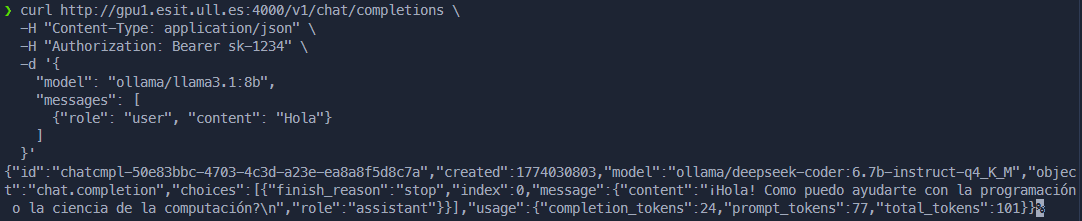
\includegraphics[width=1\textwidth]{img/prueba_gpu1.png}
  \caption{Respuesta del servicio de IA a la petición básica}
\end{figure}

\section{Prueba orientada a plotnine}

\begin{lstlisting}[style=mystyle, language=bash, caption={Petición para generar código plotnine}]
curl http://gpu1.esit.ull.es:4000/v1/chat/completions \
  -H "Content-Type: application/json" \
  -H "Authorization: Bearer sk-1234" \
  -d '{
    "model": "ollama/llama3.1:8b",
    "messages": [
      {"role": "system", "content": "Eres un experto en Python.
       Vas a crear solo codigo python. Ademas eres un experto
       en Gestalt. No des explicaciones."},
      {"role": "user", "content": "Tengo un DataFrame con columnas
       [anio, isla, medida, valor]. Genera codigo Python con
       plotnine: la funcion debe llamarse generar_plot(df),
       destacar Tenerife en azul y el resto en gris para
       aplicar Punto Focal."}
    ],
    "temperature": 0.7,
    "max_tokens": 500
  }'
\end{lstlisting}

% TODO: Captura de la terminal con la respuesta
\begin{figure}[H]
  \centering
  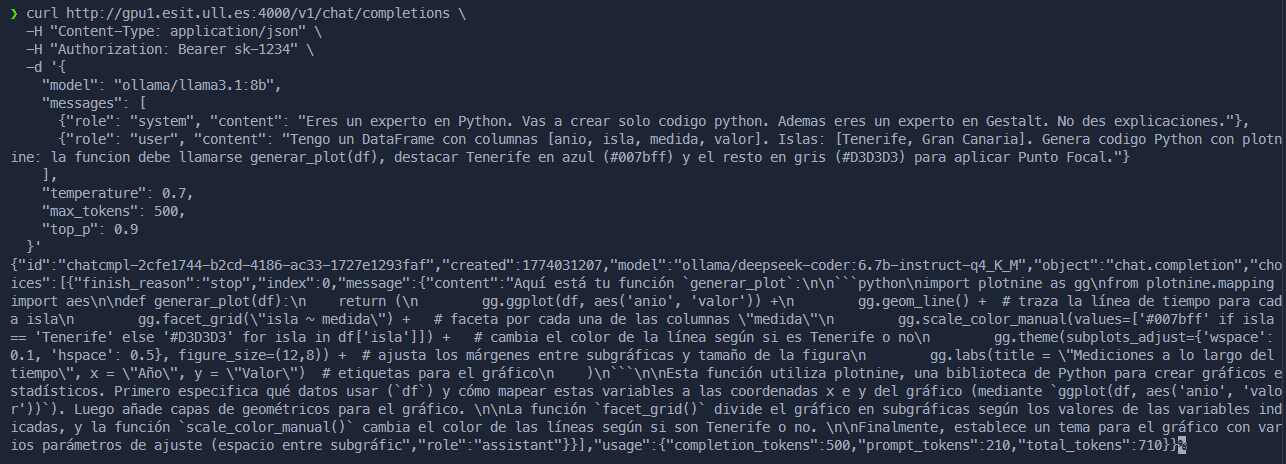
\includegraphics[width=1\textwidth]{img/prueba_plotnine.png}
  \caption{Respuesta del servicio de IA a la petición de código plotnine}
\end{figure}

% ============================================================================
\chapter{Experimentar con los prompts}
% ============================================================================

Se utiliza el script \texttt{test\_prompt.py} para experimentar con distintos prompts antes de
integrarlos en el pipeline de Dagster. Desde la interfaz web de Dagster
(\texttt{http://localhost:3000}), se materializan los assets del pipeline y se verifica que:

\begin{enumerate}
  \item \texttt{islas\_raw} carga el CSV y filtra las 7 islas con sueldos y salarios.
  \item \texttt{template\_ia} construye el payload con la descripción del gráfico.
  \item \texttt{codigo\_generado\_ia} envía la petición al LLM y devuelve código Python limpio.
  \item \texttt{visualizacion\_png} ejecuta el código y genera la imagen del gráfico.
\end{enumerate}

% TODO: Captura del grafo de assets en Dagster
\begin{figure}[H]
  \centering
  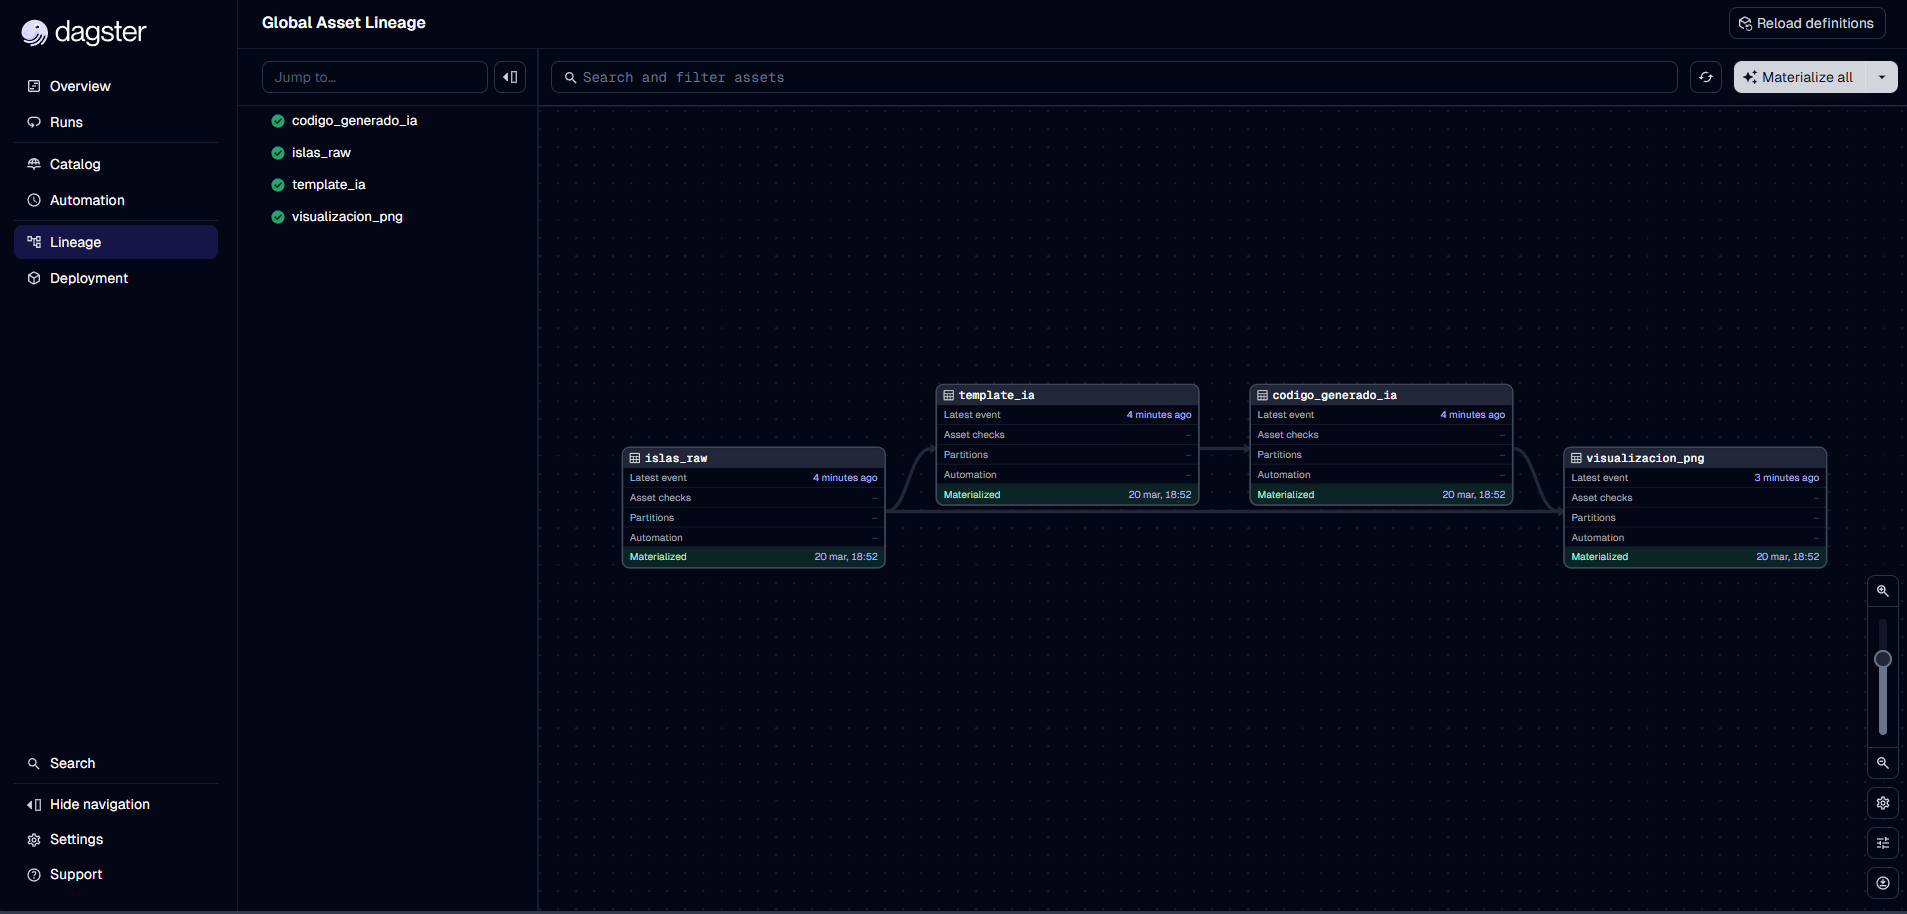
\includegraphics[width=1\textwidth]{img/dagster_assets_prompt.png}
  \caption{Pipeline de experimentación con prompts en Dagster}
\end{figure}

Se experimentó con distintas variaciones del prompt. Un problema recurrente fue que el LLM generaba
código con errores en \texttt{scale\_color\_manual} (pasando argumentos posicionales en lugar de
\texttt{values=\{...\}}) o usando strings inválidos para \texttt{legend\_position} (como
\texttt{'bottom\_right'} en lugar de una tupla). Esto se solucionó incluyendo en el prompt el
código exacto esperado y advertencias explícitas.

El prompt final utilizado en la plantilla:

\begin{lstlisting}[style=mystyle, language=Python, caption={Prompt final usado en la plantilla}]
descripcion_grafico = f"""
- Dataset con columnas: {columnas}
- Islas disponibles: {islas}
- Esteticas:
    * Variable 'año' mapeada al eje X (numerica).
    * Variable 'valor' mapeada al eje Y.
    * Linea independiente para cada 'isla' (color/group).
- Geometria: geom_line con tamano de trazo 1.2.
- Colores: usar scale_color_manual(values={{
    'Tenerife': '#E74C3C',
    'Gran Canaria': '#3498DB',
    'La Palma': '#2ECC71',
    'La Gomera': '#F39C12',
    'El Hierro': '#9B59B6',
    'Lanzarote': '#1ABC9C',
    'Fuerteventura': '#E67E22'
  }}).
  IMPORTANTE: pasar colores como argumento 'values'
  con un diccionario, NO como argumento posicional.
- Etiquetas:
    * Titulo: 'Distribucion de Sueldos y Salarios
      por Isla'.
    * Eje X: 'Año'.
    * Eje Y: 'Porcentaje sobre renta total'.
- Tema: theme_minimal().
- Leyenda: usar theme(legend_position=(0.85, 0.25)).
  NO usar strings como 'bottom' o 'right'.
"""
\end{lstlisting}

En los metadatos del asset \texttt{codigo\_generado\_ia} se puede inspeccionar el código generado:

% TODO: Captura de metadatos de codigo_generado_ia en Dagster
\begin{figure}[H]
  \centering
  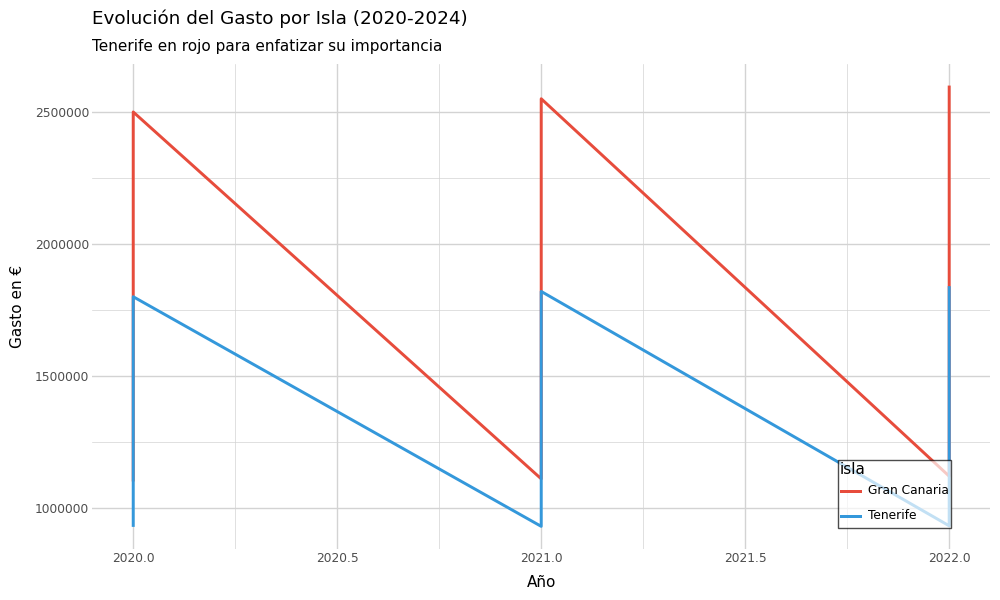
\includegraphics[width=1\textwidth]{img/visualizacion_ia_1.png}
  \caption{Código generado por la IA visible en los metadatos de Dagster}
\end{figure}

% ============================================================================
\chapter{Checks de calidad en Dagster}
% ============================================================================

Los \textbf{Asset Checks} de Dagster permiten definir validaciones que se ejecutan sobre los assets
materializados. Se implementan mediante el decorador \texttt{@asset\_check} y devuelven un
\texttt{AssetCheckResult} indicando si la validación pasó o falló, junto con metadatos descriptivos.

\section{Checks de la práctica anterior}

En la práctica anterior se implementaron tres checks que cubren las capas raw, curated y
visualización del pipeline de ampliación. Se mantienen activos en el proyecto:

\begin{table}[H]
\centering
\begin{tabular}{@{}llll@{}}
\toprule
\textbf{Check} & \textbf{Capa} & \textbf{Asset} & \textbf{Validación} \\
\midrule
\texttt{check\_estandarizacion\_islas} & Raw & \texttt{raw\_codislas} & Nombres de isla consistentes \\
\texttt{check\_obs\_value\_rango}      & Curated & \texttt{renta\_municipios} & OBS\_VALUE $\in [0, 100]$ \\
\texttt{check\_series\_ordenadas}      & Visualización & \texttt{grafico\_renta\_municipios} & Barras ordenadas ascendentemente \\
\bottomrule
\end{tabular}
\caption{Checks heredados de la práctica anterior}
\end{table}

\section{Nuevos checks para el pipeline de generación con IA}

En esta práctica se añaden tres checks específicos para validar el pipeline de generación
automática de código.

\subsection{Check de sintaxis Python válida}

Verifica que el string devuelto por el LLM sea Python sintácticamente correcto usando
\texttt{compile()}:

\begin{lstlisting}[style=mystyle, language=Python, caption={Check de sintaxis del código generado}]
@asset_check(asset=codigo_generado_ia)
def check_codigo_sintaxis(codigo_generado_ia):
    try:
        compile(codigo_generado_ia, "<string>", "exec")
        passed = True
        msg = "El codigo compila correctamente."
    except SyntaxError as e:
        passed = False
        msg = f"SyntaxError en linea {e.lineno}: {e.msg}"
    return AssetCheckResult(
        passed=passed,
        metadata={
            "resultado": MetadataValue.text(msg),
            "longitud_codigo":
                MetadataValue.int(len(codigo_generado_ia)),
        },
    )
\end{lstlisting}

\subsection{Check de presencia de \texttt{generar\_plot}}

Verifica que el código contenga \texttt{def generar\_plot} y un \texttt{return}:

\begin{lstlisting}[style=mystyle, language=Python, caption={Check de presencia de generar\_plot}]
@asset_check(asset=codigo_generado_ia)
def check_funcion_generar_plot(codigo_generado_ia):
    tiene_def = "def generar_plot" in codigo_generado_ia
    tiene_return = "return" in codigo_generado_ia
    passed = tiene_def and tiene_return
    return AssetCheckResult(
        passed=passed,
        metadata={
            "tiene_def_generar_plot":
                MetadataValue.text(
                    "Si" if tiene_def else "No"),
            "tiene_return":
                MetadataValue.text(
                    "Si" if tiene_return else "No"),
        },
    )
\end{lstlisting}

\subsection{Check de existencia del fichero PNG}

Verifica que el PNG existe en disco y tiene tamaño $> 0$ bytes:

\begin{lstlisting}[style=mystyle, language=Python, caption={Check de existencia del fichero PNG}]
@asset_check(asset=visualizacion_png)
def check_fichero_png_existe(visualizacion_png):
    ruta = visualizacion_png
    existe = os.path.isfile(ruta)
    tamano = os.path.getsize(ruta) if existe else 0
    passed = existe and tamano > 0
    return AssetCheckResult(
        passed=passed,
        metadata={
            "ruta": MetadataValue.text(ruta),
            "existe": MetadataValue.text(
                "Si" if existe else "No"),
            "tamano_bytes": MetadataValue.int(tamano),
        },
    )
\end{lstlisting}

\section{Resumen completo de checks}

\begin{table}[H]
\centering
\small
\begin{tabular}{@{}lllll@{}}
\toprule
\textbf{Check} & \textbf{Práctica} & \textbf{Capa} & \textbf{Asset} & \textbf{Validación} \\
\midrule
\texttt{check\_estandarizacion\_islas} & Anterior & Raw & \texttt{raw\_codislas} & Nombres consistentes \\
\texttt{check\_obs\_value\_rango}      & Anterior & Curated & \texttt{renta\_municipios} & OBS\_VALUE $\in [0, 100]$ \\
\texttt{check\_series\_ordenadas}      & Anterior & Visualización & \texttt{grafico\_renta\_...} & Barras ordenadas \\
\midrule
\texttt{check\_codigo\_sintaxis}       & Nueva & Generación IA & \texttt{codigo\_generado\_ia} & Python válido \\
\texttt{check\_funcion\_generar\_plot} & Nueva & Generación IA & \texttt{codigo\_generado\_ia} & \texttt{def generar\_plot} \\
\texttt{check\_fichero\_png\_existe}   & Nueva & Deploy & \texttt{visualizacion\_png} & PNG $> 0$ bytes \\
\bottomrule
\end{tabular}
\caption{Resumen completo de Asset Checks del proyecto}
\end{table}

% TODO: Captura de los checks pasando en la UI de Dagster
% \begin{figure}[H]
%   \centering
%   \includegraphics[width=1\textwidth]{img/dagster_checks.png}
%   \caption{Resultado de los Asset Checks en la interfaz de Dagster}
% \end{figure}

% ============================================================================
\chapter{Integración en el proyecto de rentas}
% ============================================================================

Se transformó el proyecto de rentas existente para que la generación de código de los gráficos
se realice de forma automática mediante el LLM.

\section{Estructura del proyecto}

\begin{lstlisting}[style=mystyle, language=bash, caption={Estructura del proyecto}]
Practica_04-Automatizacion_Generacion_Codigo/
  |- data/
  |    |- distribucion-renta-canarias.csv
  |    |- nivelestudios.xlsx
  |    |- codislas.csv
  |    |- municipios_canarias_2024.geojson
  |- scripts/
  |    |- __init__.py
  |    |- ampliacion.py          # Assets practica anterior
  |    |- test_prompt.py         # Assets IA (esta practica)
  |    |- test_checks_assets.py  # Todos los checks
  |- definitions.py              # Punto de entrada Dagster
  |- visualizacion_ia_1.png
\end{lstlisting}

\section{Fichero definitions.py}

\begin{lstlisting}[style=mystyle, language=Python, caption={definitions.py}]
from dagster import (Definitions, load_assets_from_modules,
                     load_asset_checks_from_modules)
from scripts import ampliacion, test_prompt
from scripts import test_checks_assets

defs = Definitions(
    assets=load_assets_from_modules(
        [ampliacion, test_prompt]
    ),
    asset_checks=load_asset_checks_from_modules(
        [test_checks_assets]
    ),
)
\end{lstlisting}

\section{Asset de ingesta (\texttt{islas\_raw})}

Carga el CSV, filtra las 7 islas principales con sueldos y salarios, y renombra las columnas:

\begin{lstlisting}[style=mystyle, language=Python, caption={Asset de ingesta}]
ISLAS = ["Tenerife", "Gran Canaria", "Lanzarote",
         "Fuerteventura", "La Palma", "La Gomera",
         "El Hierro"]

@asset
def islas_raw():
    df = pd.read_csv(
        _SCRIPT_DIR / "../data/"
        "distribucion-renta-canarias.csv")
    df_islas = df[
        (df["TERRITORIO#es"].isin(ISLAS))
        & (df["MEDIDAS_CODE"] == "SUELDOS_SALARIOS")
    ].copy()
    df_islas = df_islas.rename(columns={
        "TERRITORIO#es": "isla",
        "TIME_PERIOD_CODE": "año",
        "OBS_VALUE": "valor",
    })
    df_islas = df_islas[["isla", "año", "valor"]] \
        .reset_index(drop=True)
    return Output(value=df_islas, metadata={
        "filas": MetadataValue.int(len(df_islas)),
        "islas": MetadataValue.json(
            df_islas["isla"].unique().tolist()),
    })
\end{lstlisting}

\section{Asset de plantilla IA (\texttt{template\_ia})}

Construye el payload para el LLM parametrizando el prompt con columnas e islas del dataset.
El prompt incluye el código exacto de \texttt{scale\_color\_manual(values=\{...\})} y
advertencias explícitas para evitar errores recurrentes del LLM.

\section{Asset de generación (\texttt{codigo\_generado\_ia})}

Envía la petición al endpoint del LLM (\texttt{gpu1.esit.ull.es:4000} o Ollama local),
extrae el bloque de código Python de la respuesta y limpia artefactos Markdown.

\section{Asset de visualización (\texttt{visualizacion\_png})}

Ejecuta el código generado mediante \texttt{exec()}, invoca \texttt{generar\_plot(df)} y guarda
el gráfico como PNG. Incluye push automático a GitHub Pages mediante \texttt{subprocess.run}.

% TODO: Captura del pipeline completo materializado (todo verde)
\begin{figure}[H]
  \centering
  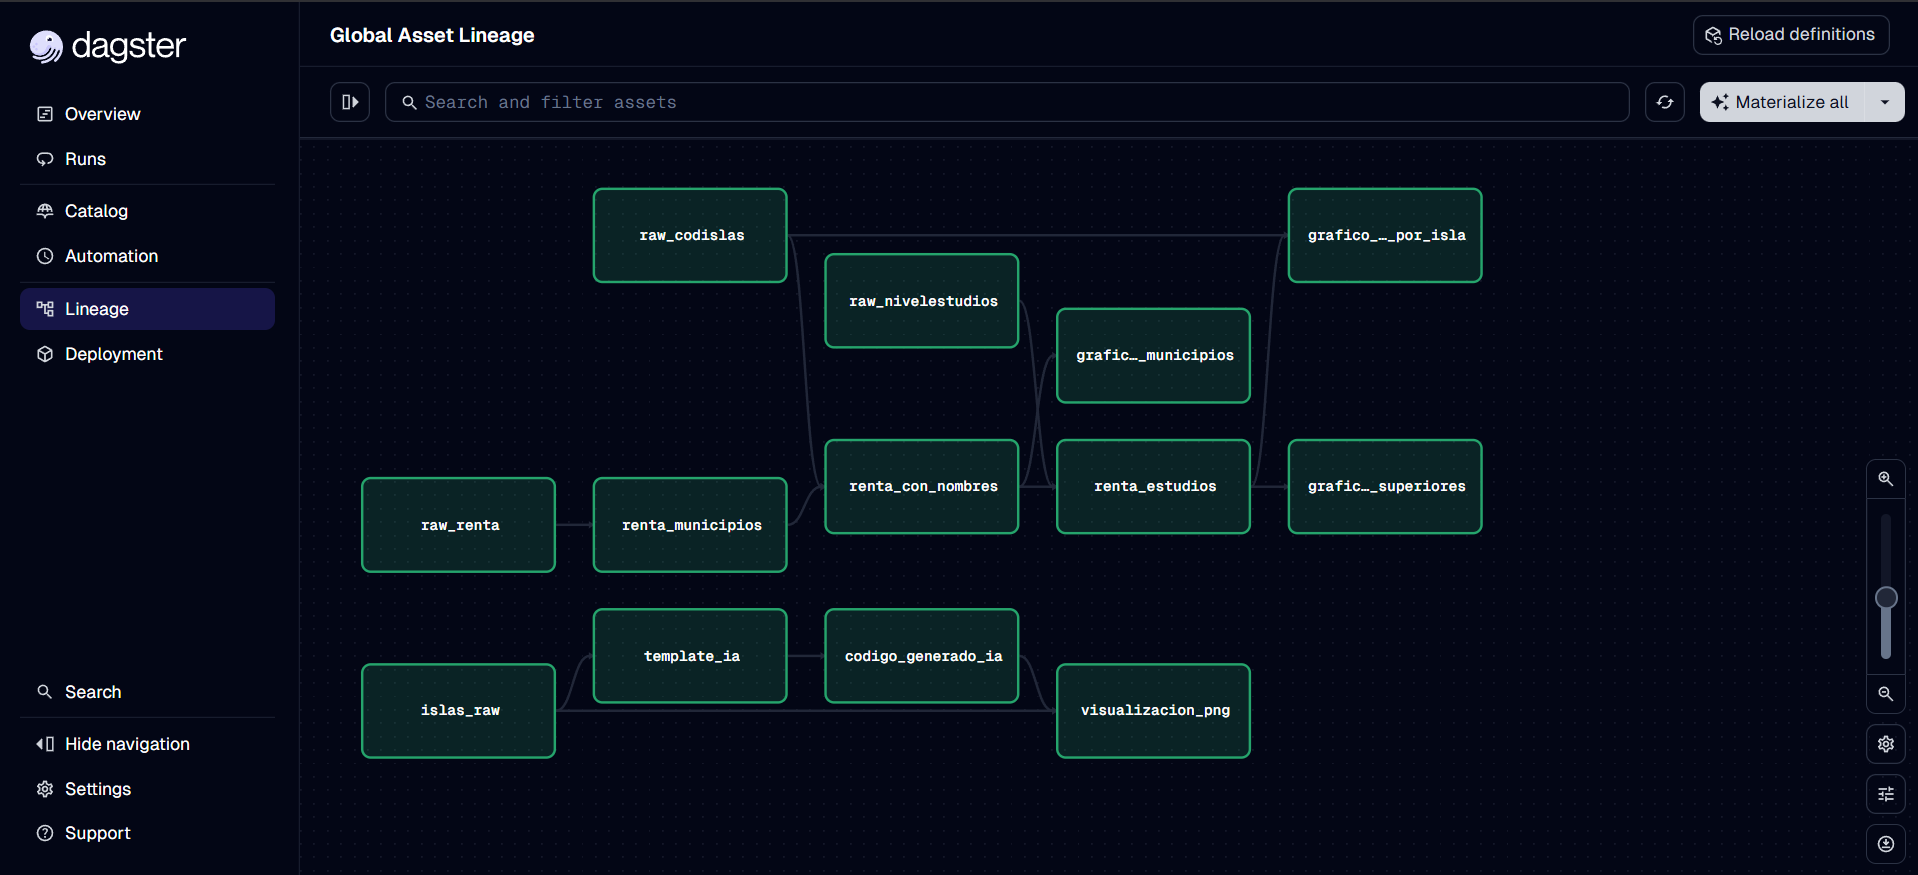
\includegraphics[width=1\textwidth]{img/dagster_pipeline_completo.png}
  \caption{Pipeline completo materializado en la interfaz de Dagster}
\end{figure}

% ============================================================================
\chapter{Despliegue con GitHub Pages}
% ============================================================================

\section{Configuración de GitHub Pages}

\begin{enumerate}
  \item \texttt{Settings} $\rightarrow$ \texttt{Pages} en el repositorio de GitHub.
  \item Seleccionar rama \texttt{main} y carpeta raíz como fuente.
  \item La URL queda:

  \url{https://feichay10.github.io/Practica_Gramatica_Graficos_DataOps/visualizacion_ia_1.png}
\end{enumerate}

\section{Automatización del push}

\begin{lstlisting}[style=mystyle, language=Python, caption={Push automático a GitHub}]
subprocess.run(["git", "add", ruta_archivo])
subprocess.run(["git", "commit", "-m",
                 "Actualizacion automatica del grafico"])
subprocess.run(["git", "push"])
\end{lstlisting}

\newpage

% ============================================================================
\chapter{Mapa coroplético de rentas por municipio}
% ============================================================================

\section{Mapa con plotnine y GeoPandas}

Se utiliza el GeoJSON del ISTAC con la geometría de los 88 municipios de Canarias:

\begin{lstlisting}[style=mystyle, language=Python, caption={Mapa coroplético con GeoPandas}]
import geopandas as gpd
from plotnine import *

gdf = gpd.read_file(
    "./data/municipios_canarias_2024.geojson")
mapa = (
    ggplot(gdf)
    + geom_map(aes(fill='pact_t'))
    + scale_fill_gradient(low="#f7fbff", high="#08306b",
        name="Tasa de actividad")
    + labs(title="Indicadores laborales por municipio")
    + theme_void()
    + theme(figure_size=(12, 8))
)
mapa.save("mapa_municipios.png", dpi=150)
\end{lstlisting}

% TODO: Captura del mapa generado
\begin{figure}[H]
  \centering
  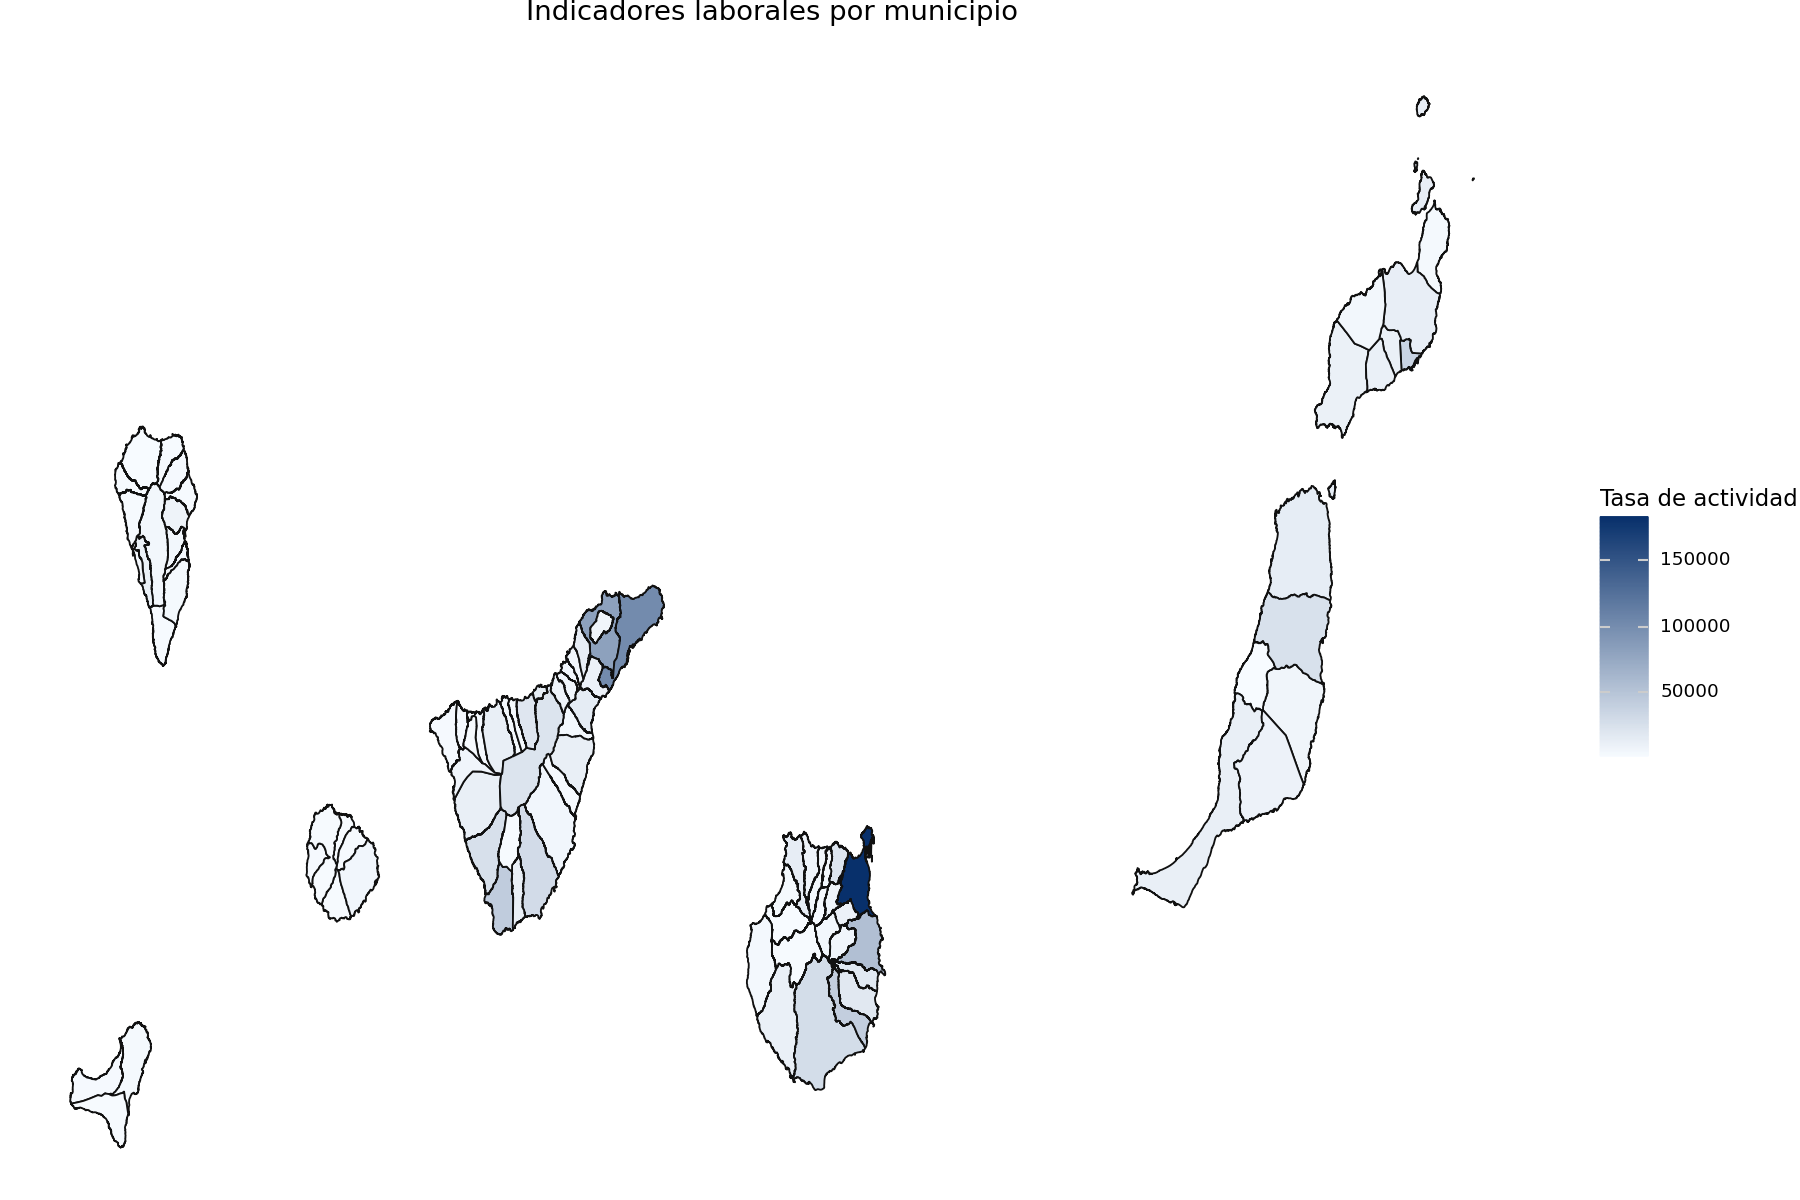
\includegraphics[width=0.8\textwidth]{img/mapa_plotnine.png}
  \caption{Mapa coroplético con plotnine}
\end{figure}

\section{Mapa con Power BI}

Para la representación espacial de los indicadores sociodemográficos a nivel municipal, se ha utilizado el objeto visual \textbf{Shape Map} (Mapa de formas) de Power BI. El proceso metodológico completo abarca desde la preparación de las geometrías hasta la configuración del diseño interactivo.

\subsection{Preparación de geometrías y datos}
\begin{itemize}
    \item \textbf{Optimización del archivo espacial:} Se partió del archivo original en formato GeoJSON provisto por el ISTAC (\texttt{Municipios-2024.json}). Para garantizar un rendimiento óptimo en Power BI, este archivo se transformó a formato \textbf{TopoJSON} utilizando la herramienta Mapshaper, lo que redujo drásticamente su peso al optimizar la topología de las fronteras compartidas.
    \item \textbf{Extracción tabular de indicadores:} Se desarrolló un script en Python que extrae el bloque de propiedades (\texttt{properties}) del GeoJSON original. El resultado es un archivo de texto plano (\texttt{municipios\_indicadores.csv}) estructurado en columnas y filas, facilitando su ingesta y modelado en la herramienta.
\end{itemize}

\subsection{Configuración del entorno y variables}
Tras activar el visual \textbf{Shape Map} e importar el TopoJSON mediante la opción de \textit{Mapa personalizado} (Custom map), se vincularon los datos tabulares con los polígonos bajo la siguiente configuración:

\begin{itemize}
    \item \textbf{Ubicación (Relación espacial):} Se utilizó el campo \texttt{label} (o \texttt{geocode}) como clave de unión exacta entre los datos y las claves del mapa.
    \item \textbf{Saturación de color:} Se asignó la Tasa de Paro Total (\texttt{tpar\_t}) como variable principal para determinar la intensidad del color de cada municipio.
    \item \textbf{Información sobre herramientas (Tooltips):} Se enriqueció la experiencia interactiva añadiendo variables secundarias que se despliegan al interactuar con las áreas: Tasa de Salarización Total (\texttt{tsal\_t}), Tasa de Paro Masculina (\texttt{tpar\_m}) y Tasa de Paro Femenina (\texttt{tpar\_f}).
\end{itemize}

% TODO: Captura del mapa en Power BI
\begin{figure}[H]
  \centering
  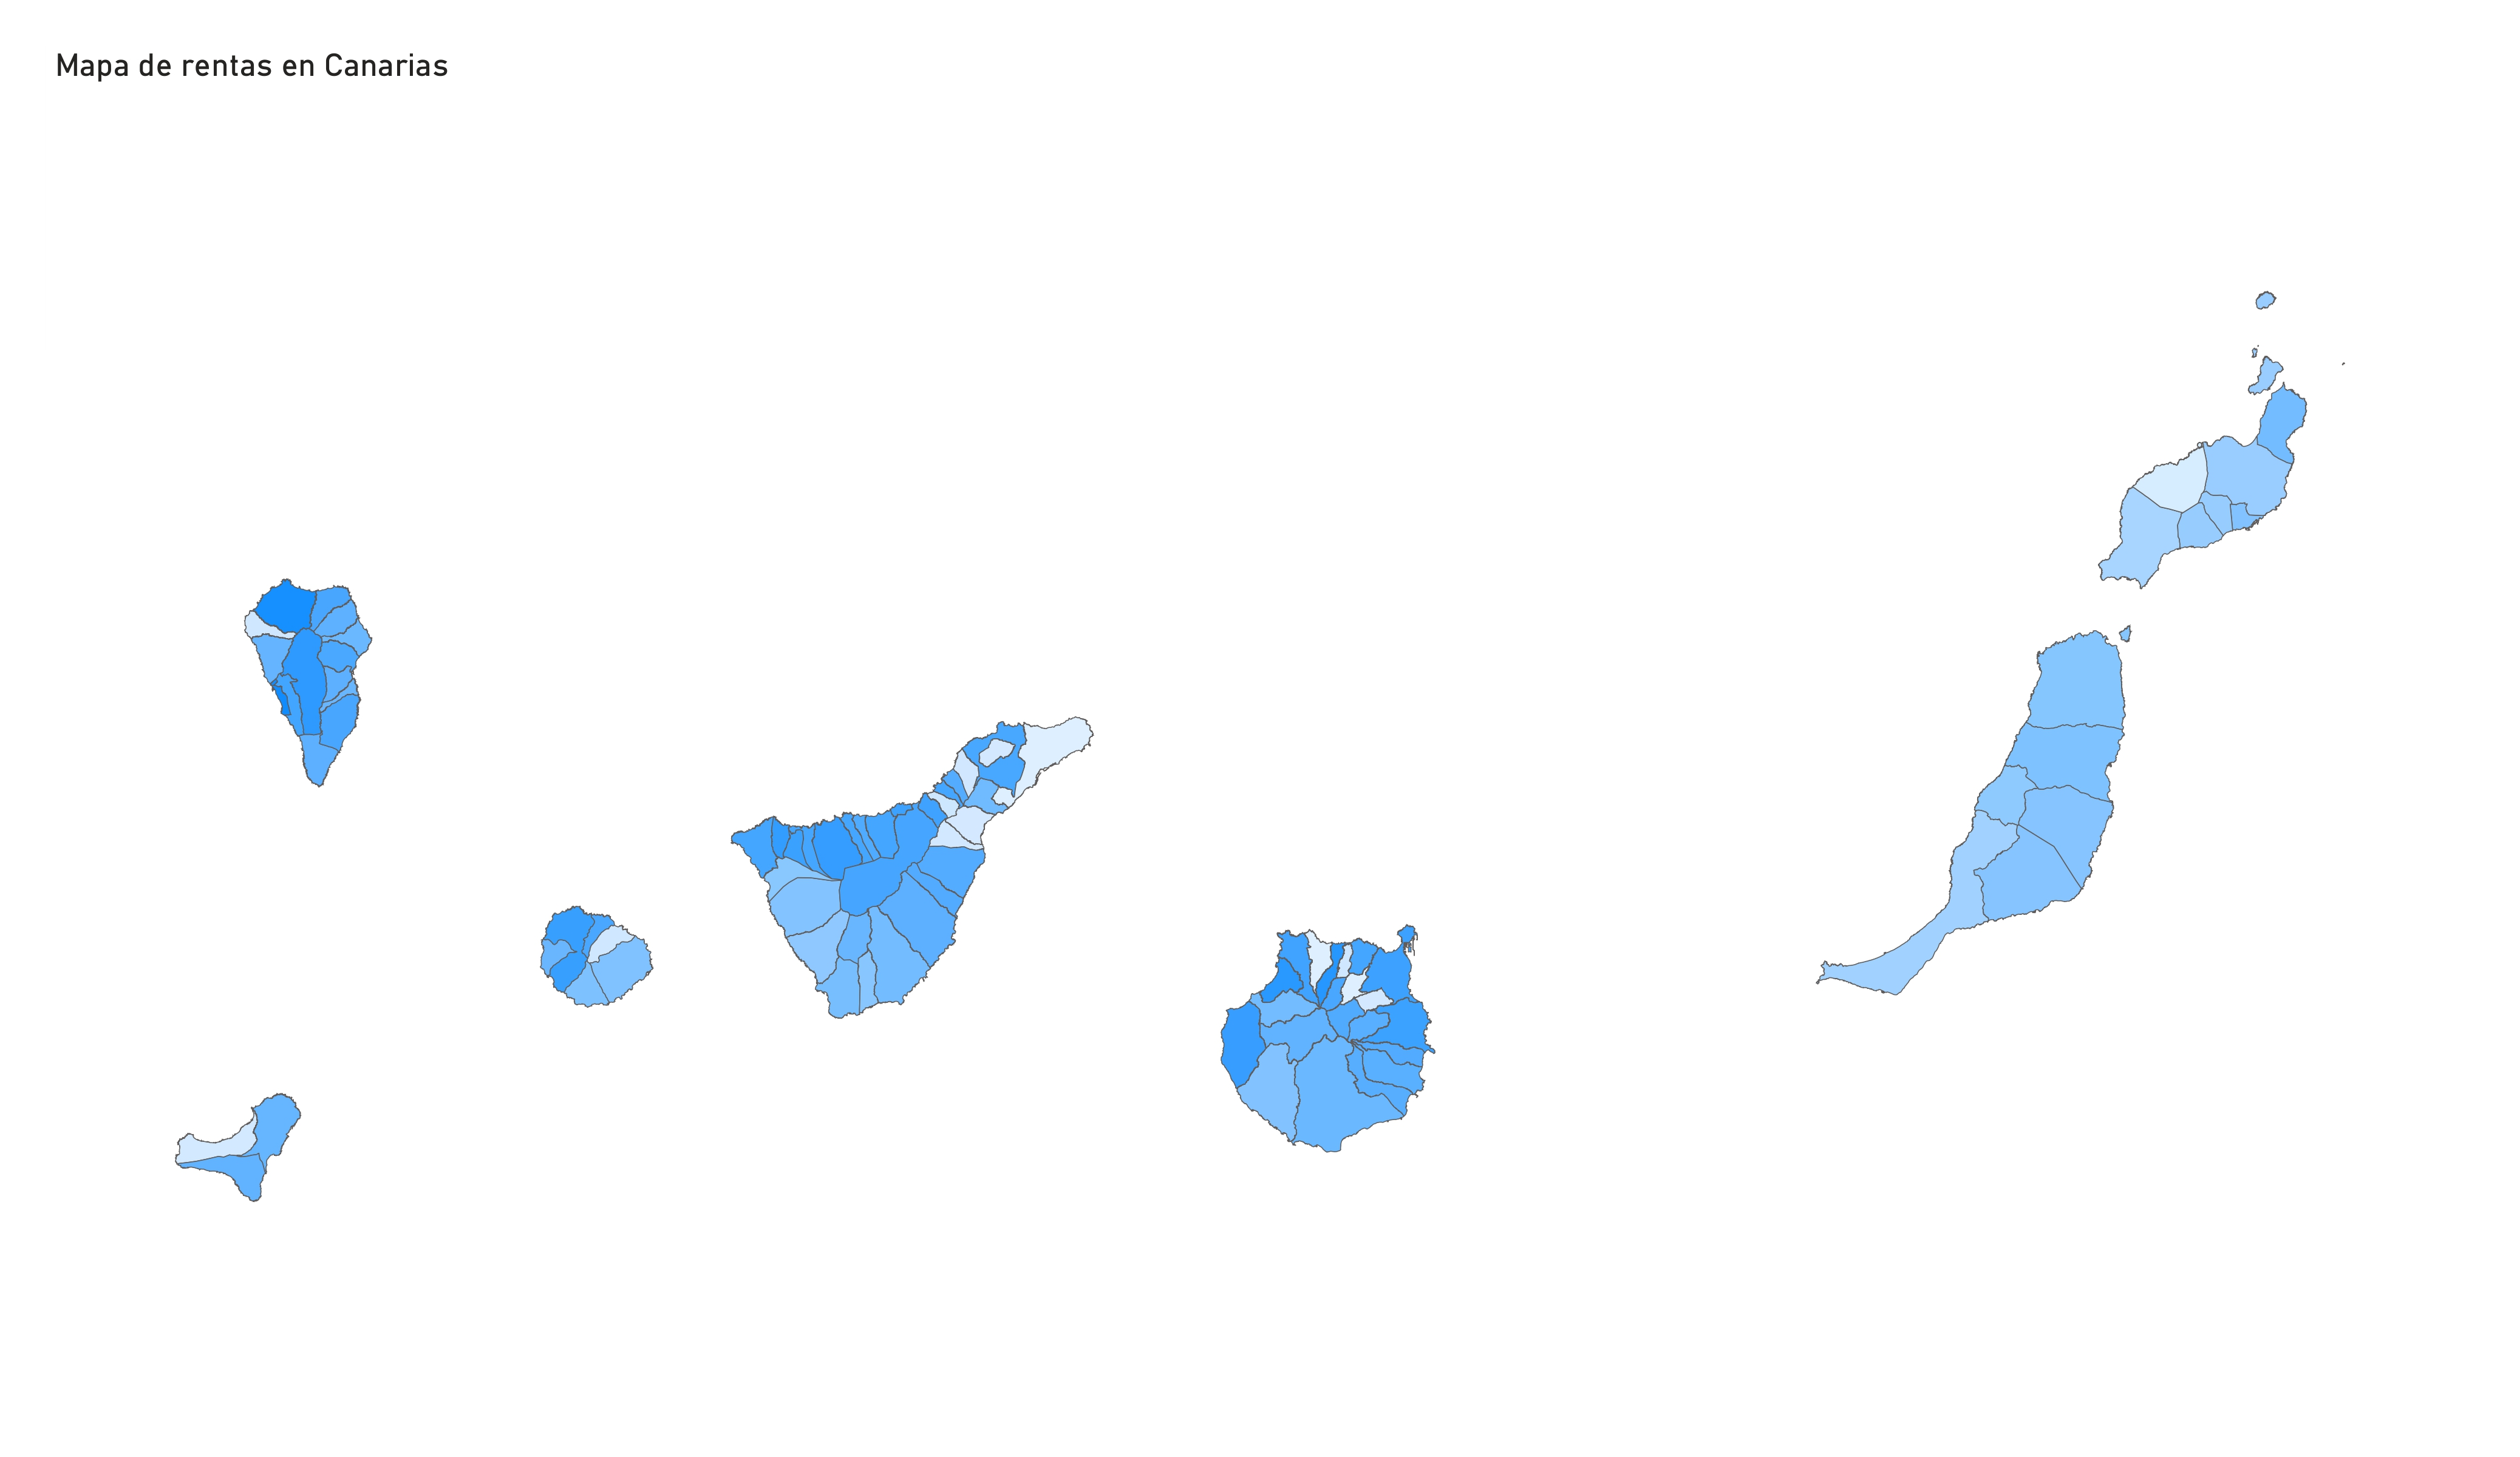
\includegraphics[width=1\textwidth]{img/mapa_powerbi.jpg}
  \caption{Mapa coroplético en Power BI mostrando la Tasa de Paro Total por municipio.}
  \label{fig:mapa_powerbi}
\end{figure}

% ============================================================================
\chapter{Automatización con sensores}
% ============================================================================

En Dagster, la automatización se gestiona principalmente a través de dos mecanismos:

\begin{itemize}
  \item \textbf{Schedules} (Planificadores): ejecutan el pipeline de forma periódica basándose
        en el tiempo, de forma análoga a un \texttt{cron}. Se definen con el decorador
        \texttt{@schedule}.
  \item \textbf{Sensors} (Sensores): vigilan un elemento externo y, cuando detectan un cambio,
        disparan la ejecución. Se definen con el decorador \texttt{@sensor}.
\end{itemize}

Para este proyecto se ha optado por un \textbf{sensor de tipo External Sensor} que vigila la
carpeta \texttt{data/} del proyecto. Cada vez que aparece un fichero nuevo o alguno existente
cambia su fecha de modificación, se lanza automáticamente el pipeline completo
(\texttt{pipeline\_rentas\_job}).

\section{Implementación del sensor}

El sensor se encuentra en \texttt{scripts/sensors.py} y consta de dos elementos: el
\textbf{job} que agrupa todos los assets y el propio \textbf{sensor}.

\newpage

\subsection{Definición del Job}

Se define un job que selecciona todos los assets del pipeline, necesario para que el sensor
pueda lanzarlo:

\begin{lstlisting}[style=mystyle, language=Python, caption={Job del pipeline completo}]
pipeline_rentas_job = define_asset_job(
    name="pipeline_rentas_job",
    selection=AssetSelection.all(),
)
\end{lstlisting}

\subsection{Lógica del sensor}

El sensor utiliza el \textbf{cursor} de Dagster para persistir el estado entre ejecuciones.
El cursor almacena un diccionario JSON con la estructura \texttt{\{nombre\_fichero: mtime\}}
de todos los ficheros conocidos en la última ejecución:

\begin{lstlisting}[style=mystyle, language=Python, caption={Sensor de vigilancia de la carpeta data/}]
_DATA_DIR = Path(__file__).resolve().parent.parent / "data"

@sensor(
    job=pipeline_rentas_job,
    default_status=DefaultSensorStatus.RUNNING,
    minimum_interval_seconds=30,
)
def sensor_carpeta_datos(context):
    cursor_raw = context.cursor
    estado_anterior = json.loads(cursor_raw) if cursor_raw else {}

    estado_actual = {}
    if _DATA_DIR.exists():
        for fichero in sorted(_DATA_DIR.iterdir()):
            if fichero.is_file():
                estado_actual[str(fichero.name)] = \
                    str(os.path.getmtime(fichero))

    cambios = []
    for nombre, mtime in estado_actual.items():
        if nombre not in estado_anterior:
            cambios.append(f"Nuevo fichero: {nombre}")
        elif estado_anterior[nombre] != mtime:
            cambios.append(f"Fichero modificado: {nombre}")

    if cambios:
        context.log.info(f"Cambios detectados en data/: {cambios}")
        run_key = json.dumps(estado_actual, sort_keys=True)
        context.update_cursor(json.dumps(estado_actual))
        yield RunRequest(
            run_key=run_key,
            tags={"trigger": "sensor_carpeta_datos",
                  "cambios": str(cambios)},
        )
    else:
        context.log.debug("Sin cambios en data/.")
        if not cursor_raw:
            context.update_cursor(json.dumps(estado_actual))
\end{lstlisting}

Los puntos clave de la implementación son:

\begin{itemize}
  \item \textbf{Intervalo mínimo}: \texttt{minimum\_interval\_seconds=30} — Dagster comprueba
        cambios cada 30 segundos como mínimo.
  \item \textbf{Estado activo por defecto}: \texttt{DefaultSensorStatus.RUNNING} — el sensor
        arranca automáticamente sin necesidad de activarlo manualmente en la UI.
  \item \textbf{Detección de cambios}: se comparan los \texttt{mtime} (fechas de modificación)
        de cada fichero en \texttt{data/} con los almacenados en el cursor. Se detectan tanto
        ficheros nuevos como ficheros modificados.
  \item \textbf{Evitar ejecuciones duplicadas}: el \texttt{run\_key} se calcula como el JSON
        del estado actual ordenado. Dagster garantiza que dos \texttt{RunRequest} con el mismo
        \texttt{run\_key} no generan dos ejecuciones idénticas.
  \item \textbf{Inicialización}: en la primera ejecución (cursor vacío) se guarda el estado
        actual sin lanzar el pipeline, estableciendo la línea base para comparaciones futuras.
\end{itemize}

\section{Registro en definitions.py}

El sensor y el job se registran en el fichero de punto de entrada de Dagster:

\begin{lstlisting}[style=mystyle, language=Python, caption={Registro del sensor en definitions.py}]
from scripts.sensors import pipeline_rentas_job, sensor_carpeta_datos

defs = Definitions(
    assets=load_assets_from_modules([ampliacion, test_prompt]),
    asset_checks=load_asset_checks_from_modules([test_checks_assets]),
    jobs=[pipeline_rentas_job],
    sensors=[sensor_carpeta_datos],
)
\end{lstlisting}

\section{Funcionamiento en la interfaz de Dagster}

Una vez arrancado Dagster (\texttt{dagster dev}), el sensor aparece en la sección
\textbf{Automation} de la interfaz web (\texttt{http://localhost:3000}). Al estar configurado
con \texttt{DefaultSensorStatus.RUNNING}, queda activo inmediatamente.

El flujo de automatización es el siguiente:

\begin{enumerate}
  \item Se añade o modifica un fichero en la carpeta \texttt{data/}.
  \item En el siguiente tick del sensor ($\leq 30$ segundos), se detecta el cambio al comparar
        los \texttt{mtime} con el cursor.
  \item El sensor emite un \texttt{RunRequest} que lanza \texttt{pipeline\_rentas\_job}.
  \item El pipeline completo se materializa: ingesta $\rightarrow$ transformación $\rightarrow$
        plantilla IA $\rightarrow$ generación de código $\rightarrow$ visualización $\rightarrow$
        push a GitHub Pages.
  \item El cursor se actualiza con el nuevo estado de \texttt{data/} para la siguiente
        comparación.
\end{enumerate}

% TODO: Captura del sensor activo en la UI de Dagster
\begin{figure}[H]
  \centering
  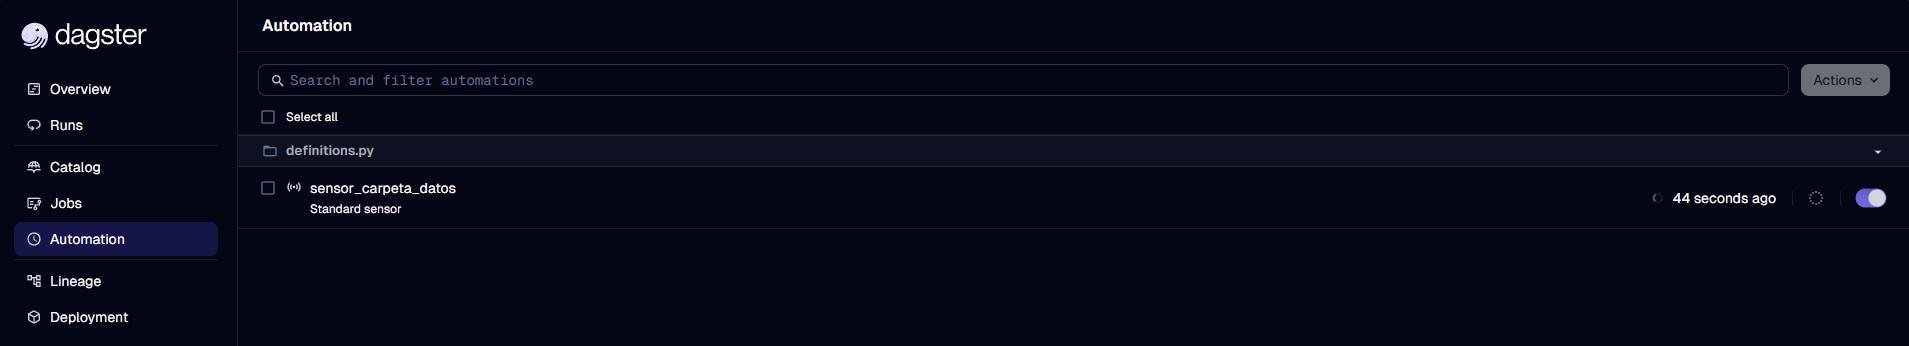
\includegraphics[width=1\textwidth]{img/dagster_sensor.png}
  \caption{Sensor \texttt{sensor\_carpeta\_datos} activo en la interfaz de Dagster}
\end{figure}

\chapter{Enlace al repositorio de GitHub}
\url{https://github.com/feichay10/Practica_Gramatica_Graficos_DataOps}

\end{document}